\documentclass[11pt,preprint, authoryear]{elsarticle}

\usepackage{lmodern}
%%%% My spacing
\usepackage{setspace}
\setstretch{1.2}
\DeclareMathSizes{12}{14}{10}{10}

% Wrap around which gives all figures included the [H] command, or places it "here". This can be tedious to code in Rmarkdown.
\usepackage{float}
\let\origfigure\figure
\let\endorigfigure\endfigure
\renewenvironment{figure}[1][2] {
    \expandafter\origfigure\expandafter[H]
} {
    \endorigfigure
}

\let\origtable\table
\let\endorigtable\endtable
\renewenvironment{table}[1][2] {
    \expandafter\origtable\expandafter[H]
} {
    \endorigtable
}


\usepackage{ifxetex,ifluatex}
\usepackage{fixltx2e} % provides \textsubscript
\ifnum 0\ifxetex 1\fi\ifluatex 1\fi=0 % if pdftex
  \usepackage[T1]{fontenc}
  \usepackage[utf8]{inputenc}
\else % if luatex or xelatex
  \ifxetex
    \usepackage{mathspec}
    \usepackage{xltxtra,xunicode}
  \else
    \usepackage{fontspec}
  \fi
  \defaultfontfeatures{Mapping=tex-text,Scale=MatchLowercase}
  \newcommand{\euro}{€}
\fi

\usepackage{amssymb, amsmath, amsthm, amsfonts}

\def\bibsection{\section*{References}} %%% Make "References" appear before bibliography


\usepackage[round]{natbib}

\usepackage{longtable}
\usepackage[margin=2.3cm,bottom=2cm,top=2.5cm, includefoot]{geometry}
\usepackage{fancyhdr}
\usepackage[bottom, hang, flushmargin]{footmisc}
\usepackage{graphicx}
\numberwithin{equation}{section}
\numberwithin{figure}{section}
\numberwithin{table}{section}
\setlength{\parindent}{0cm}
\setlength{\parskip}{1.3ex plus 0.5ex minus 0.3ex}
\usepackage{textcomp}
\renewcommand{\headrulewidth}{0.2pt}
\renewcommand{\footrulewidth}{0.3pt}

\usepackage{array}
\newcolumntype{x}[1]{>{\centering\arraybackslash\hspace{0pt}}p{#1}}

%%%%  Remove the "preprint submitted to" part. Don't worry about this either, it just looks better without it:
\makeatletter
\def\ps@pprintTitle{%
  \let\@oddhead\@empty
  \let\@evenhead\@empty
  \let\@oddfoot\@empty
  \let\@evenfoot\@oddfoot
}
\makeatother

 \def\tightlist{} % This allows for subbullets!

\usepackage{hyperref}
\hypersetup{breaklinks=true,
            bookmarks=true,
            colorlinks=true,
            citecolor=blue,
            urlcolor=blue,
            linkcolor=blue,
            pdfborder={0 0 0}}


% The following packages allow huxtable to work:
\usepackage{siunitx}
\usepackage{multirow}
\usepackage{hhline}
\usepackage{calc}
\usepackage{tabularx}
\usepackage{booktabs}
\usepackage{caption}


\newenvironment{columns}[1][]{}{}

\newenvironment{column}[1]{\begin{minipage}{#1}\ignorespaces}{%
\end{minipage}
\ifhmode\unskip\fi
\aftergroup\useignorespacesandallpars}

\def\useignorespacesandallpars#1\ignorespaces\fi{%
#1\fi\ignorespacesandallpars}

\makeatletter
\def\ignorespacesandallpars{%
  \@ifnextchar\par
    {\expandafter\ignorespacesandallpars\@gobble}%
    {}%
}
\makeatother

\newenvironment{CSLReferences}[2]{%
}

\urlstyle{same}  % don't use monospace font for urls
\setlength{\parindent}{0pt}
\setlength{\parskip}{6pt plus 2pt minus 1pt}
\setlength{\emergencystretch}{3em}  % prevent overfull lines
\setcounter{secnumdepth}{5}

%%% Use protect on footnotes to avoid problems with footnotes in titles
\let\rmarkdownfootnote\footnote%
\def\footnote{\protect\rmarkdownfootnote}
\IfFileExists{upquote.sty}{\usepackage{upquote}}{}

%%% Include extra packages specified by user

%%% Hard setting column skips for reports - this ensures greater consistency and control over the length settings in the document.
%% page layout
%% paragraphs
\setlength{\baselineskip}{12pt plus 0pt minus 0pt}
\setlength{\parskip}{12pt plus 0pt minus 0pt}
\setlength{\parindent}{0pt plus 0pt minus 0pt}
%% floats
\setlength{\floatsep}{12pt plus 0 pt minus 0pt}
\setlength{\textfloatsep}{20pt plus 0pt minus 0pt}
\setlength{\intextsep}{14pt plus 0pt minus 0pt}
\setlength{\dbltextfloatsep}{20pt plus 0pt minus 0pt}
\setlength{\dblfloatsep}{14pt plus 0pt minus 0pt}
%% maths
\setlength{\abovedisplayskip}{12pt plus 0pt minus 0pt}
\setlength{\belowdisplayskip}{12pt plus 0pt minus 0pt}
%% lists
\setlength{\topsep}{10pt plus 0pt minus 0pt}
\setlength{\partopsep}{3pt plus 0pt minus 0pt}
\setlength{\itemsep}{5pt plus 0pt minus 0pt}
\setlength{\labelsep}{8mm plus 0mm minus 0mm}
\setlength{\parsep}{\the\parskip}
\setlength{\listparindent}{\the\parindent}
%% verbatim
\setlength{\fboxsep}{5pt plus 0pt minus 0pt}



\begin{document}



\begin{frontmatter}  %

\title{Question 3: Portfolio Construction}

% Set to FALSE if wanting to remove title (for submission)




\author[Add1]{Gabriella Neilon}
\ead{22581340@sun.ac.za}





\address[Add1]{Stellenbosch University}

\cortext[cor]{Corresponding author: Gabriella Neilon}

\begin{abstract}
\small{
This article examines the methodologies of the SWIX and ALSI indexes,
focusing on various aspects such as size indexes (large, mid, and small
caps), sector exposures, and stock concentration over time. Using a
comprehensive analysis of Exchange Rate data, it highlights the
differences in return profiles of both methodologies during periods of
currency performance and volatility.

Additionally, the study responds to the JSE's inquiry on the impact of
applying different capping levels (e.g., 5\%, 10\%, and uncapped) to the
SWIX and ALSI. Utilizing data from Rebalance days.rds to identify past
quarterly rebalances, it assesses the effects of various capping levels
on both indexes.

Key findings reveal that Large Capped funds tend to outperform Mid and
Small Capped Funds, albeit demonstrating higher overall volatility.
Furthermore, the ALSI generally outperforms the SWIX in terms of
returns, although both exhibit relatively similar volatility levels.
Notably, within the SWIX index, the returns of Large and Mid capped
funds demonstrate close alignment, suggesting a correlation in their
performance trends.

Moreover, the research highlights that both SWIX and ALSI encounter
increased volatility during periods of high exchange rate volatility,
with SWIX displaying more significant effects than ALSI. This pattern
remains consistent even during low volatility periods.

Interestingly, ALSI exhibits higher sensitivity to capping constraints
compared to SWIX. Despite this, ALSI consistently outperforms SWIX
across various restrictions. This suggests that ALSI might require more
nuanced management or adjustments to adhere to specific limitations
without compromising its performance.
}
\end{abstract}

\vspace{1cm}





\vspace{0.5cm}

\end{frontmatter}

\setcounter{footnote}{0}



%________________________
% Header and Footers
%%%%%%%%%%%%%%%%%%%%%%%%%%%%%%%%%
\pagestyle{fancy}
\chead{}
\rhead{}
\lfoot{}
\rfoot{\footnotesize Page \thepage}
\lhead{}
%\rfoot{\footnotesize Page \thepage } % "e.g. Page 2"
\cfoot{}

%\setlength\headheight{30pt}
%%%%%%%%%%%%%%%%%%%%%%%%%%%%%%%%%
%________________________

\headsep 35pt % So that header does not go over title




\hypertarget{basic-comparison-of-different-capped-funds-for-alsi-and-swix}{%
\section{Basic comparison of different `Capped' funds for ALSI and
SWIX}\label{basic-comparison-of-different-capped-funds-for-alsi-and-swix}}

The data showcases that Large Capped funds outperform both Mid and Small
Capped Funds, although they also tend to demonstrate higher overall
volatility. Within the ALSI index, the returns exceed those observed in
the SWIX index. However, both ALSI and SWIX exhibit relatively similar
volatility.

Regarding the SWIX index, the returns of Large and Mid capped funds seem
to be more closely aligned with each other. This suggests a degree of
correlation or similarity in the performance trend between the Large and
Mid capped funds within the SWIX index.

\hypertarget{alsi}{%
\subsection{ALSI}\label{alsi}}

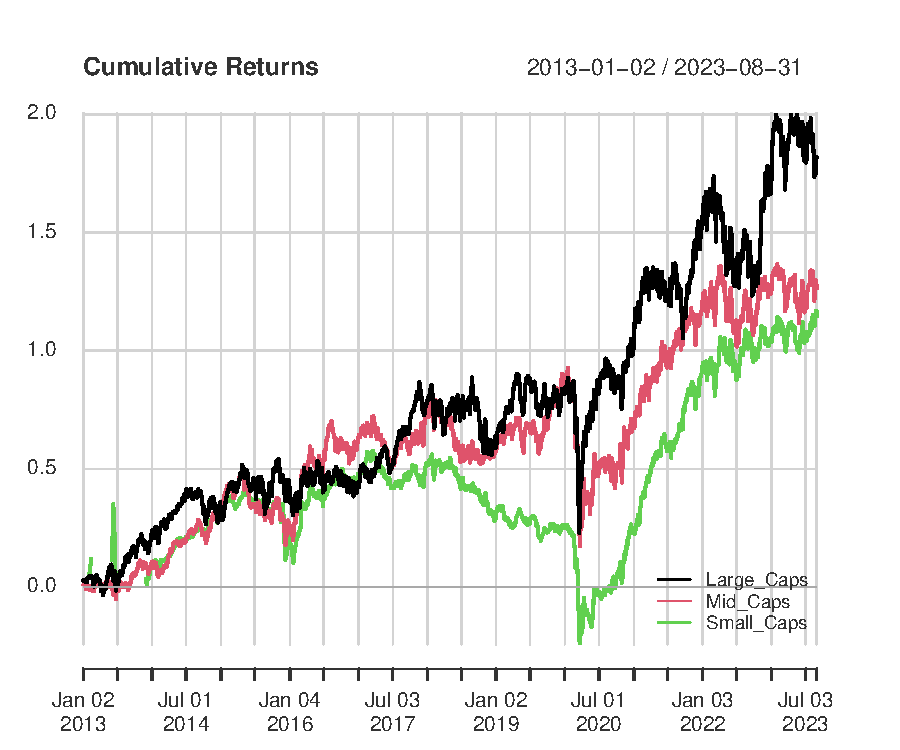
\includegraphics{Question-3_files/figure-latex/unnamed-chunk-1-1.pdf}

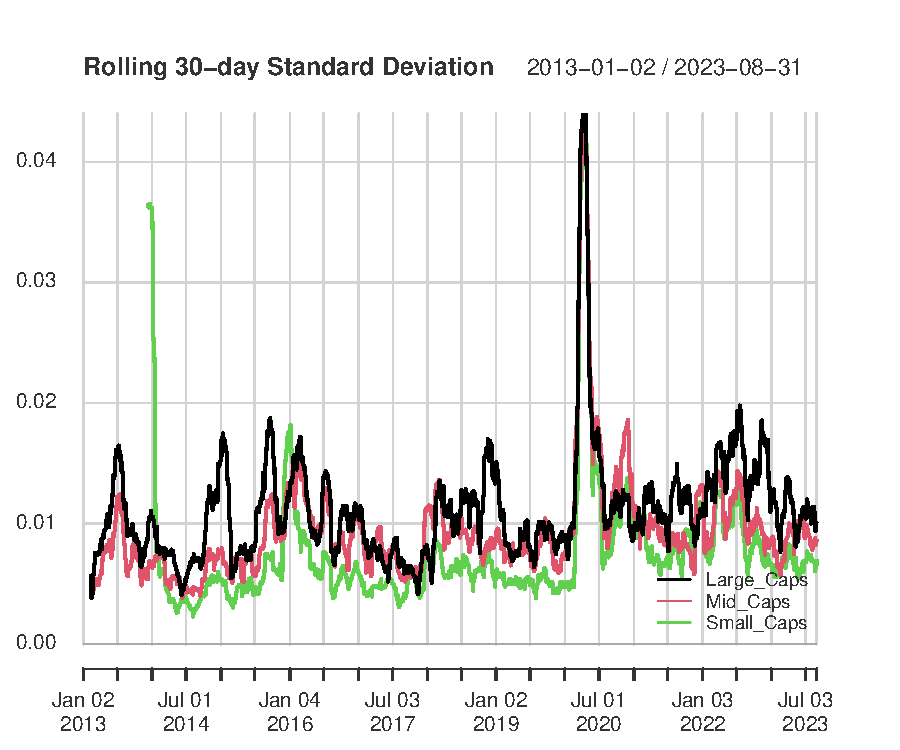
\includegraphics{Question-3_files/figure-latex/unnamed-chunk-2-1.pdf}

\hypertarget{swix}{%
\subsection{SWIX}\label{swix}}

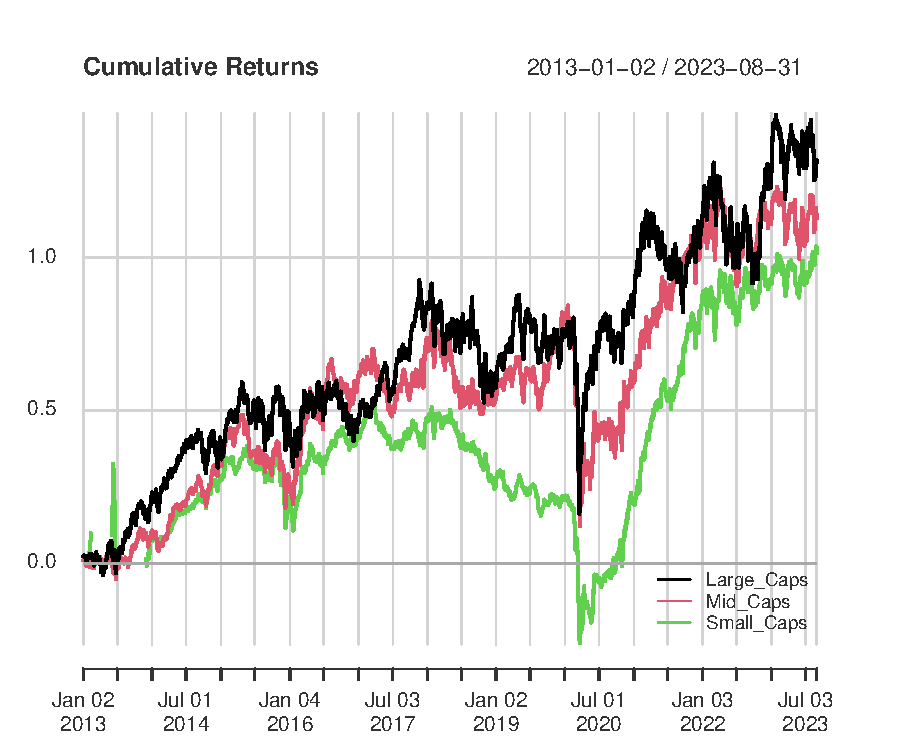
\includegraphics{Question-3_files/figure-latex/unnamed-chunk-3-1.pdf}

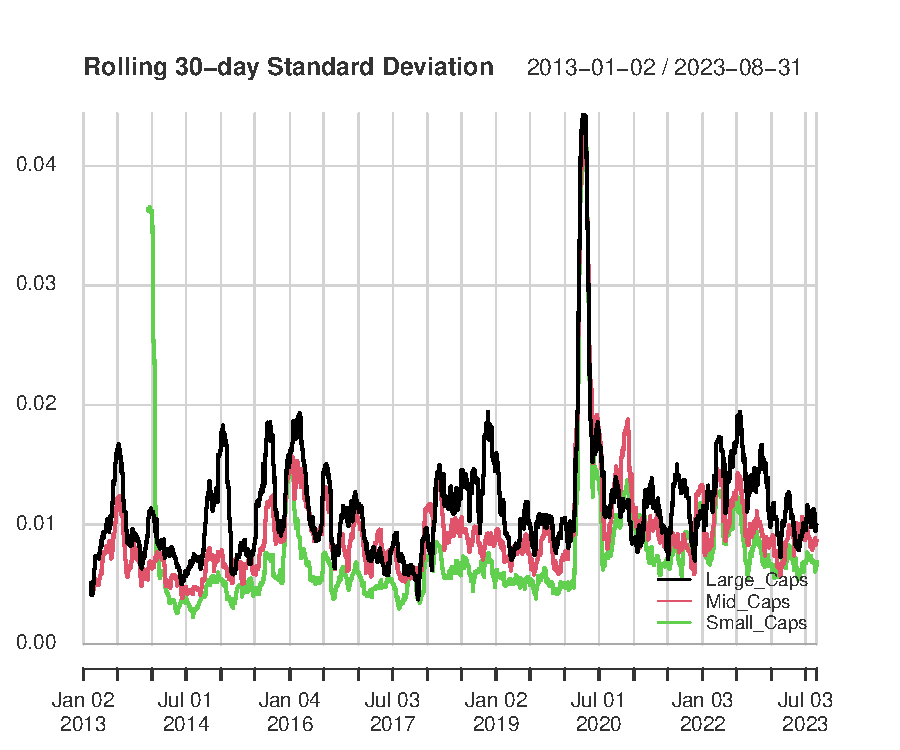
\includegraphics{Question-3_files/figure-latex/unnamed-chunk-4-1.pdf}

\hypertarget{periods-of-high-and-low-volatility}{%
\section{Periods of high and low
volatility}\label{periods-of-high-and-low-volatility}}

\begin{verbatim}
## # A tibble: 3 x 5
## # Groups:   Index [3]
##   Index              SD Full_SD Period   Ratio
##   <chr>           <dbl>   <dbl> <chr>    <dbl>
## 1 ZAR.USD.Return 0.191   0.141  High_Vol 1.35 
## 2 SWIX           0.0428  0.0366 High_Vol 1.17 
## 3 ALSI           0.0337  0.0344 High_Vol 0.981
\end{verbatim}

\begin{verbatim}
## # A tibble: 3 x 5
## # Groups:   Index [3]
##   Index              SD Full_SD Period  Ratio
##   <chr>           <dbl>   <dbl> <chr>   <dbl>
## 1 ZAR.USD.Return 0.104   0.141  Low_Vol 0.740
## 2 SWIX           0.0286  0.0366 Low_Vol 0.781
## 3 ALSI           0.0266  0.0344 Low_Vol 0.775
\end{verbatim}

These tables demonstrates that during periods of high exchange rate
volatility, both SWIX and ALSI experience increased volatility, with
SWIX being more significantly affected compared to ALSI. This pattern
holds true during low volatility periods as well.

\hypertarget{capping}{%
\section{Capping}\label{capping}}

The figure illustrates that ALSI is more sensitive to the imposition of
capping constraints compared to SWIX. Despite this higher
susceptibility, ALSI consistently outperforms SWIX across all three
restrictions.

This implies that even with the imposition of constraints, ALSI manages
to maintain better performance than SWIX. The sensitivity of ALSI to
these restrictions suggests it might require more nuanced management or
adjustments to adhere to certain limitations without compromising its
performance.
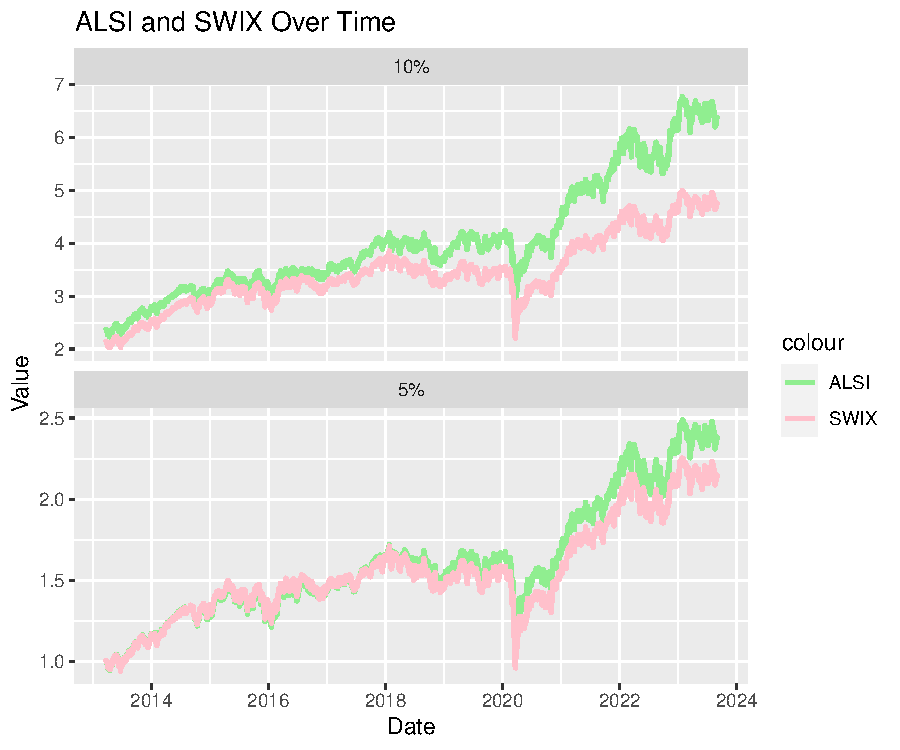
\includegraphics{Question-3_files/figure-latex/unnamed-chunk-9-1.pdf}

\hfill

\newpage

\bibliography{Tex/ref}





\end{document}
